\section{Введение}

\textbf{Цели работы:}

1) Экспериментально получить зависимость между напряжением
и деформацией (закон Гука) для одноосного растяжения
результатам измерений вычислить модуль Юнга.

2) Измерение углов закручивания в зависимости от приложенного
момента сил, расчет модулей кручения и сдвига при
статическом закручивании стержня, определение тех же модулей
для проволоки по измерениям периодов крутильных колебаний
подвешенного на ней маятника (динамическим методом).

\textbf{В работе используются:}
в первой части: прибор Лермантова, проволока из исследуемого
материала, зрительная труба со шкалой, набор грузов,
микрометр, рулетка; во второй части: исследуемый стержень,
отсчетная труба со шкалой, рулетка, микрометр, набор грузов;
в третьей части: проволока из исследуемого материала, грузы,
секундо-мер, микрометр, рулетка, линейка.

\subsection{Определение модуля Юнга по измерениям растяжения проволоки}
\begin{figure}[H]
    \centering
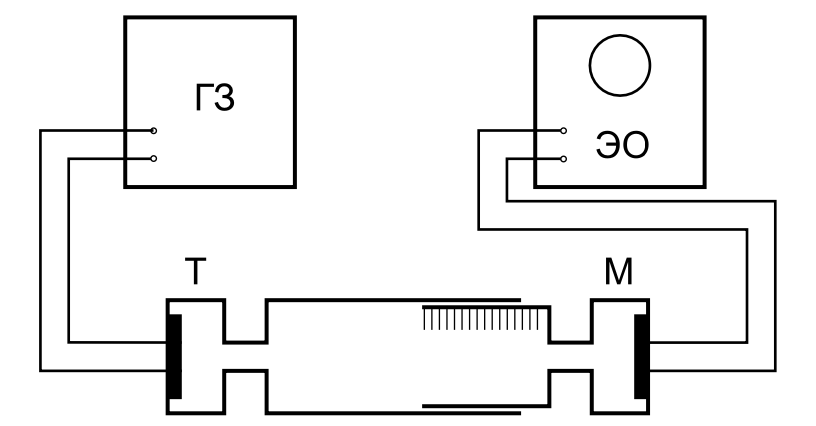
\includegraphics[width=0.5\linewidth,center]{p1.png}
    \caption{Прибор Лермантова}
    \label{fig:my_label}
\end{figure}
В первой части работы производят растяжение проволоки,
и это соответствует случаю одноосного напряженного состояния,
описываемого формулой
\[\sigma = E\varepsilon.\]
Для определения модуля Юнга используется прибор Лермантова,
схема которого изображена на рис. 1. Верхний конец проволоки
П, изготовленной из исследуемого материала, прикреплен к
консоли К, а нижний - к цилиндру, которым оканчивается
шарнирный кронштейн III. На этот же цилиндр опирается рычаг $r$,
связанный с зеркальцем 3. Таким образом, удлинение проволоки
можно измерить по углу поворота зеркальца.

Натяжение проволоки можно менять, перекладывая грузы с
площадки М на площадку О и наоборот. Такая система позволяет
исключить влияние деформации кронштейна К на точность
измерений, так как нагрузка на нем все время остается
постоянной.

При проведении эксперимента следует иметь в виду, что проволока
П при отсутствии нагрузки всегда несколько изогнута, что не может не сказаться на результатах, особенно при небольших нагрузках. Проволока вначале не столько растягивается, сколько распрямляется.


\subsection{Определение модуля кручения}

При закручивании цилиндрических стержней круглого сечения
распределение деформаций и напряжений одинаково по длине
стержня только вдали от мест, где прикладываются закручивающие
моменты. Для этих областей можно считать, что каждое
поперечное сечение поворачивается как жесткое, то есть
частички материала не сходят с тех радиальных линий, на
которых они находились вначале, и все эти радиальные линии
поворачиваются на один и тот же угол. Напряженное состояние,
которое при этом возникает, называется чистым кручением. Далее
будет показано, что касательные напряжения в поперечном
сечении увеличиваются пропорционально расстоянию от оси
вращения.


Рассмотрим часть закручиваемого круглого цилиндра, имеющую
длину $l$, которая изображена на рис. 2а. Любая прямая линия,
проведенная до закручивания цилиндра по частицам материала и
параллельная оси симметрии, при закручивании превращается в
спираль (винтовую линию). Сечения, находящиеся на расстоянии
$l$, повернуты на угол $\varphi$.

Для вывода основных соотношений, описывающих кручение, удобно
рассмотреть в цилиндре колечко произвольного радиуса $r$ с
бесконечно малой толщиной $dr$ и бесконечно малой высотой $dl$
показанное на рис. 2б. При закручивании верхнее сечение
колечка поворачивается относительно нижнего на угол
$d\varphi$, а образующая цилиндрической поверхности колечка
$dl$ наклоняется на угол $\alpha$, представляя элемент тех
спиральных линий, о которых говорилось выше. При небольших
углах а можно написать
\begin{equation}
    \alpha dl = rd\varphi.
\end{equation}

Видно, что $\alpha$ возрастет с увеличением расстояния от оси
цилиндра $r$. На рис. 2в показан элемент колечка, вмороток
происходит сдвиговая деформация. Касательное напряжение $\tau$
связано с углом сдвига $\alpha$ линейной зависимостью, в
которую входит модуль сдвига $ G$:
\begin{equation}
    \tau = G\alpha.
\end{equation}
\begin{figure}[H]
    \centering
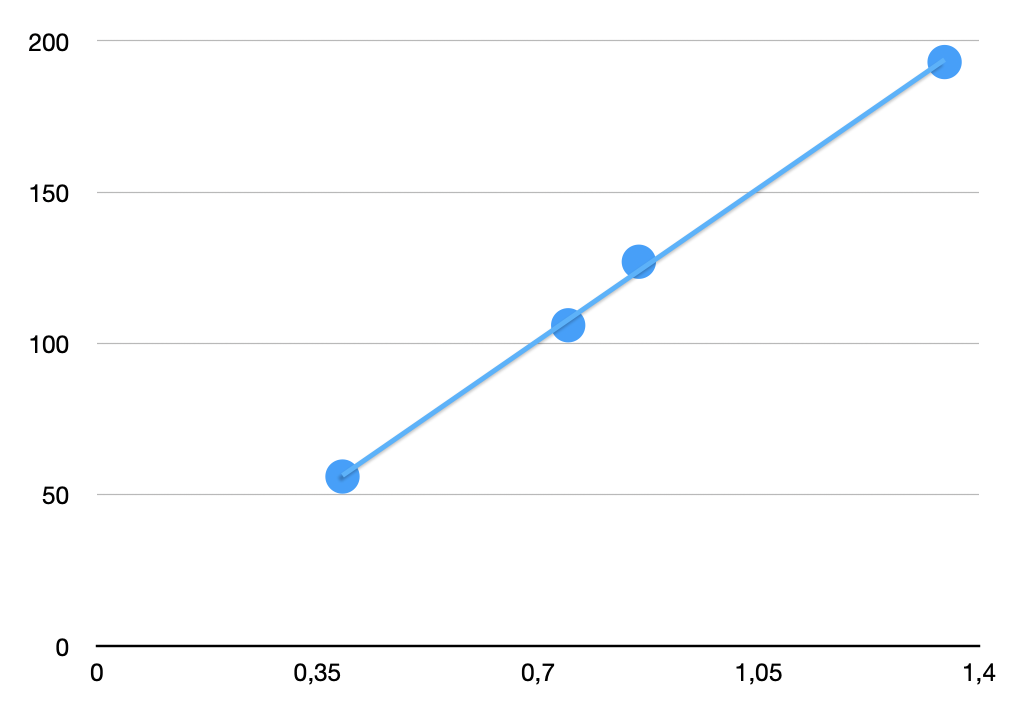
\includegraphics[width=0.5\linewidth,center]{p2.png}
    \caption{Закручивание цилиндра}
    \label{fig:my_label}
\end{figure}

Касательное напряжение $\tau$ пропорционально $\alpha$,
следовательно, тоже растет с увеличением расстояния то оси
цилиндра, о чем уже говорилось выше. Используя (1),
получаем
\begin{equation}
    \tau = Gr\frac{d\varphi}{dl}.
\end{equation}

Эти касательные напряжения создают момент сил относительно
оси цилиндра:
\begin{equation}
    dM = 2\pi rdr\cdot \tau \cdot r.
\end{equation}

Суммарный момент сил, действующий на всем поперечном сечении
цилиндра, находится интегрированием по колечкам от оси
цилиндра до его радиуса $R$:
\begin{equation}
    M = 2\pi G\frac{d\varphi}{dl}\int\limits_0^R r^3dr =
    \pi G\frac{d\varphi}{dl}\frac{R^4}{2}.
\end{equation}

Этот момент не меняется по длине цилиндра. Моменты на торцах
любой выделенной части цилиндра уравновешивают друг друга
(нет вращения цилиндра). При этом из (5) следует линейная
зависимость между относительным поворотом поперечных сечений
цилиндра --  углом $\varphi$ и расстоянием $l$, на котором
они находятся. Таким образом, для связи приложенного момента
сил $M$ и угла поворота $\varphi$ поперечных сечений цилиндра
$\varphi$, находящихся на расстоянии $l$, получаем
\begin{equation}
    M = \frac{\pi R^4G}{2l}\varphi = f\varphi.
\end{equation}

Здесь введен модуль кручения $f$, связанный с модулем
сдвига $G$:
\begin{equation}
    f = \frac{\pi R^4 G}{2l}.
\end{equation}

Необходимо подчеркнуть, что зависимость (6) выполняется при
напряжениях намного меньших модуля сдвига, то есть при малых
углах $\alpha$.
\subsubsection{Статический метод}
Схема экспериментальной установки для статического
закручивания стержня изображена на рис.3. Верхний конец
вертикально расположенного стержня С жестко закреплен на
стойке, а нижний соединен с диском Д. Момент $М$,
закручивающий стержень, создают две навитые на диск и
перекинутые через блоки Б нити, к концам которых
подвешиваются одинаковые грузы Г. Диск снабжен зеркальцем 3.
Для определения угла закручивания стержня надо лазер
направить на зеркальце и снять измерения, на которое будет
показывать лазерный луч.
\begin{figure}[H]
    \centering
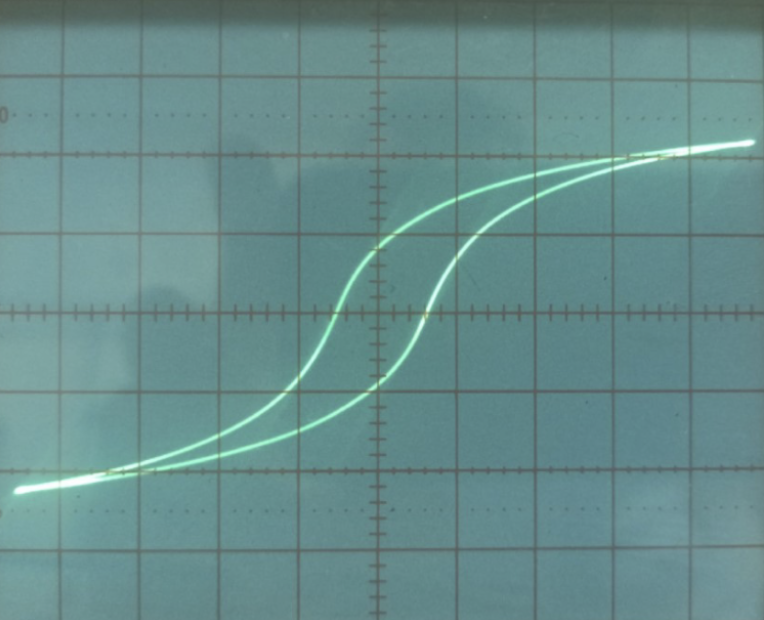
\includegraphics[width=0.5\linewidth,center]{p3.png}
    \caption{Схема для статического метода}
    \label{fig:my_label}
\end{figure}
\subsubsection{Крутильные колебания}
Экспериментальная установка, используемая в этой части работы,
изображена на рис. 4 и состоит из длинной вертикально висящей
проволоки П, к нижнему концу которой прикреплен
горизонтальный металлический стержень С с двумя симметрично
расположенными грузами Г. Их положение на стержне можно
фиксировать. Верхний конец проволоки зажат в цангу и при
помощи специального приспособления может вместе с цангой
поворачиваться вокруг вертикальной оси. Таким способом в
системе можно возбуждать крутильные колебания. Вращение
стержня С с закрепленными на нем грузами Г вокруг
вертикальной оси происходит под действием упругого момента,
возникающего в проволоке. Это вращение описывается уравнением:
\begin{equation}
    I\frac{d^2\varphi}{dt^2} = - M.
\end{equation}
Здесь $I$ - момент инерции стержня с грузами относительно оси
вращения, $\varphi$ - угол поворота стержня от положения
равновесия, М - момент сил, действующий на стержень при
закручивании проволоки, который при малых закручиваниях
(малых $\varphi$) описывается формулой (6).
Вводим обозначение:
\begin{equation}
    \omega^2 = \frac fI.
\end{equation}
При этом из (6) и (8) получаем:
\begin{equation}
    \frac{d^2\varphi}{dt^2} + \omega^2\varphi = 0.
\end{equation}
Период колебаний Т равен
\begin{equation}
    T = \frac{2\pi}{\omega} = 2\pi\sqrt\frac If.
\end{equation}
Уравнение (10) и, следовательно, (11) и получены для
незатухающих колебаний. Для их применения необходимо
убедиться, что в рассматриваемом случае затуханием колебаний,
то есть необратимыми потерями энергии, можно пренебречь. Если
после 10 периодов колебаний амплитуда уменьшается меньше, чем
в 2 раза, то можно пользоваться результатами для незатухающих
колебаний. Кроме того, следуех убедиться, что период
колебаний не зависих от начальной амплитуды. Начальную
амплитуду нужно уменьшахь до тех пор, пока не исчезает
зависимость периода от амплитуды.
\begin{figure}[H]
    \centering
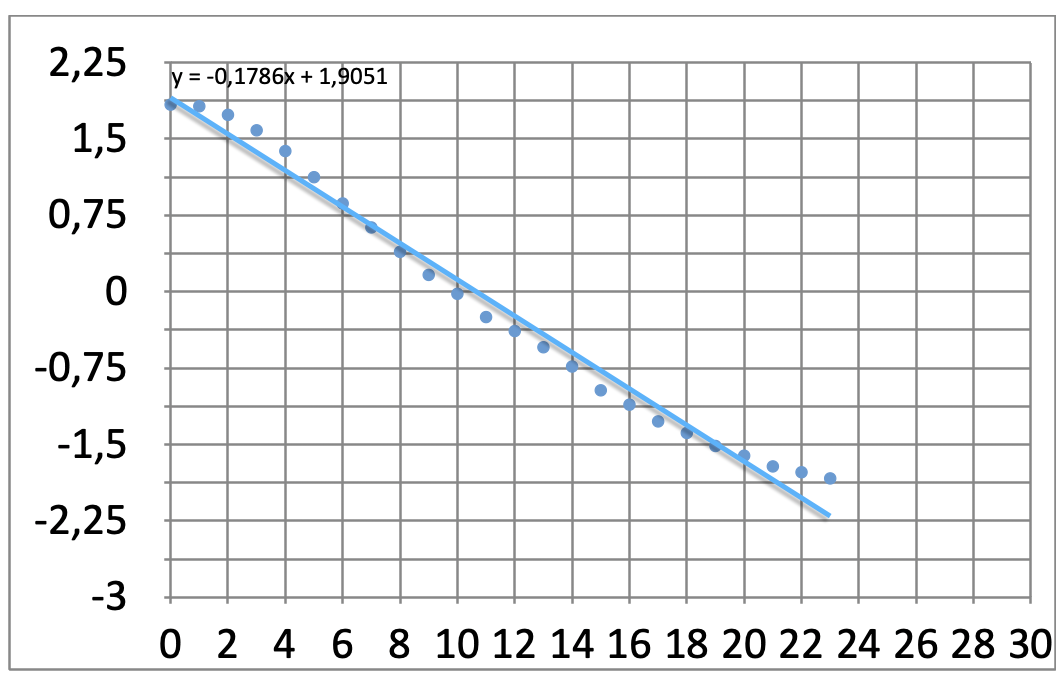
\includegraphics[width=0.5\linewidth,center]{p4.png}
    \caption{Установка для круттильных колебаний}
    \label{fig:my_label}
\end{figure}
